\documentclass[aspectratio=169, table]{beamer}

\usepackage{colortbl}
\usepackage{xcolor}
\usepackage{listings}
\usepackage{tikz}
\usepackage{pgfplots}
\usepgfplotslibrary{polar}
\usetikzlibrary{arrows.meta, positioning, calc}

\usetheme{Pradita}



\lstdefinelanguage{bash} {
	keywords={},
	basicstyle=\ttfamily\small,
	keywordstyle=\color{blue}\bfseries,
	ndkeywords={iex},
	ndkeywordstyle=\color{purple}\bfseries,
	sensitive=true,
	commentstyle=\color{gray},
	stringstyle=\color{red},
	numbers=left,
	numberstyle=\tiny\color{gray},
	breaklines=true,
	frame=lines,
	backgroundcolor=\color{lightgray!10},
	tabsize=2,
	comment=[l]{\#},
	morecomment=[s]{/*}{*/},
	commentstyle=\color{gray}\ttfamily,
	stringstyle=\color{purple}\ttfamily,
	showstringspaces=false
}

% Define Python language style for listings
\lstdefinestyle{PythonStyle}{
    language=Python,
    basicstyle=\ttfamily\footnotesize,
    keywordstyle=\color{blue}\bfseries,
    commentstyle=\color{gray}\itshape,
    stringstyle=\color{red},
    showstringspaces=false,
    breaklines=true,
    frame=lines,
    numbers=left,
    numberstyle=\tiny\color{gray},
    backgroundcolor=\color{lightgray!10},
    tabsize=4,
    captionpos=b
}


\title{\Huge Running Systems \\
	\vspace{10pt}
	before Design}
\subtitle{IT30213 - Advanced Software Engineering \& DevOps}
%\date[Serial]{Penggunaan Large Language Model untuk Pengajaran}
\author{\textbf{Alfa Yohannis}}
\begin{document}
	
	\frame{\titlepage}
	

	\begin{frame}[fragile]
		\frametitle{Contents}
		\vspace{20pt}
		\begin{columns}[t]
			\column{0.5\textwidth}
			\tableofcontents[sections={1-5}]
			
			\column{0.5\textwidth}
			\tableofcontents[sections={6-20}]
		\end{columns}
	\end{frame}
	
	\begin{frame}{\hfill}
		\centering
		\Huge{\textbf{What are Software Systems and\\how to make them work?}}
	\end{frame}
	
	\section{Introduction}
	
	\begin{frame}{\hfill}
		\centering
		\Huge{\textbf{Introduction}}
	\end{frame}
	

\begin{frame}{Course Introduction}
	\vspace{20pt}
	\begin{itemize}
		\item Modern software systems are large, distributed, and continuously running across diverse environments.
		\item Understanding such systems requires reasoning across \textbf{execution, configuration, and automation}, not code alone.
		\item This course begins from \textbf{running systems} and progressively moves toward abstraction and design.
		\item Runtime behaviour is treated as the primary source of evidence for system understanding.
		\item Models and languages are introduced as \textbf{executable artefacts} that control, generate, and automate systems.
		\item The course bridges software engineering, DevOps, and model-driven engineering into a single execution-centred view.
	\end{itemize}
\end{frame}

\begin{frame}{Required Software}
	\vspace{10pt}
	\begin{columns}[t]
		\column{0.52\textwidth}
		\textbf{Core (Required)}
		\vspace{6pt}
		\begin{itemize}
			\item \textbf{Docker} (container runtime)
			\item \textbf{Docker Compose} (multi-container orchestration)
			\item \textbf{Python 3.12} (runtime for system nodes)
			\item \textbf{Web Browser} (to view MJPEG stream)
		\end{itemize}
		
		\vspace{6pt}
		\textbf{Recommended}
		\vspace{6pt}
		\begin{itemize}
			\item \textbf{Visual Studio Code} (editor + integrated terminal)
			\item VS Code extensions: \textbf{Python}, \textbf{Docker}
		\end{itemize}
		
		\column{0.44\textwidth}
		\textbf{Optional (Local / Non-containerized)}
		\vspace{6pt}
		\begin{itemize}
			\item \textbf{Python Virtual Environments} (\texttt{venv})
			\item \textbf{pip} (package installer)
		\end{itemize}
		
		\vspace{10pt}
		\textbf{Platforms}
		\vspace{6pt}
		\begin{itemize}
			\item Windows / macOS / Linux (Ubuntu recommended for CLI work)
		\end{itemize}
	\end{columns}
	
	\vspace{6pt}
	{\footnotesize Goal: a consistent runtime environment for executing Broker + Node A + Node B + Node C}
\end{frame}


\section{Course Session Overview}
\begin{frame}{Course Sessions Overview}
	\begin{columns}[t]
		\column{0.5\textwidth}
		\begin{enumerate}
			\item \textbf{Session-01}. Running Systems Before Design
			\item \textbf{Session-02}. Observability Before Architecture
			\item \textbf{Session-03}. Runtime Control, Security, and Policies
			\item \textbf{Session-04}. CI/CD and Script Explosion
			\item \textbf{Session-05}. Runtime Models and Executable Behavior
			\item \textbf{Session-06}. Metamodeling Fundamentals
			\item \textbf{Session-07}. Textual DSL Engineering
		\end{enumerate}
		
		\column{0.5\textwidth}
		\begin{enumerate}
			\setcounter{enumi}{7}
			\item \textbf{Session-08}. Visual Language Engineering for Runtime Models
			\item \textbf{Session-09}. Projectional Language Engineering
			\item \textbf{Session-10}. Semantic Design of Executable Models
			\item \textbf{Session-11}. Model-to-Model Transformation and Refinement
			\item \textbf{Session-12}. Constraints and Model Validation
			\item \textbf{Session-13}. Model-to-Text Generation and DevSecOps Execution
		\end{enumerate}
		{\scriptsize Running systems to automated systems generation}
	\end{columns}
\end{frame}

\begin{frame}{Introduction of This Session}
	\vspace{10pt}
	\begin{itemize}
		\item Software systems are first encountered as \textbf{running artefacts}, not as diagrams or models.
		\item Observable behaviour emerges from execution, configuration, and environment, rather than from design alone.
		\item Understanding begins by \textbf{running, modifying, and observing} a real system in operation.
		\item Behaviour-first interaction builds intuition about data flow, dependencies, and failure modes.
		\item Design, architecture, and models are introduced later as tools to \textbf{explain and control} observed behaviour.
	\end{itemize}
	
	\vspace{6pt}
	{\footnotesize This session grounds abstraction in concrete runtime experience}
\end{frame}

	\begin{frame}{\hfill}
		\centering
		\Huge{\textbf{Demo}}
	\end{frame}

\section{Runtime Structure of the Example System}
\begin{frame}{Runtime Structure of the Example System}
	\vspace{20pt}
	\centering
	\scalebox{1.1}{
	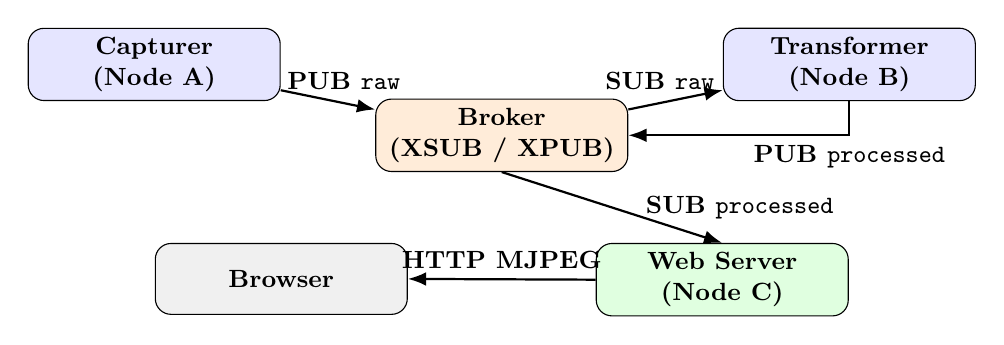
\begin{tikzpicture}[
		font=\small\bfseries,
		node distance=9mm and 12mm,
		box/.style={
			draw,
			rounded corners=2mm,
			align=center,
			minimum width=32mm,
			minimum height=9mm,
			fill=blue!10
		},
		brokerbox/.style={box,fill=orange!15},
		webbox/.style={box,fill=green!12},
		browserbox/.style={box,fill=gray!12},
		arrow/.style={-Latex,thick}
	]
	
	\node[brokerbox] (broker) {Broker\\(XSUB / XPUB)};
	\node[box,left=of broker,yshift=+9mm] (capturer) {Capturer\\(Node A)};
	\node[box,right=of broker,yshift=+9mm] (transformer) {Transformer\\(Node B)};
	
	\node[webbox,below=of broker,xshift=+28mm] (web) {Web Server\\(Node C)};
	\node[browserbox,below=of broker,xshift=-28mm] (browser) {Browser};
	
	\draw[arrow] (capturer) -- node[above,xshift=2mm]{PUB \texttt{raw}} (broker);
	\draw[arrow] (broker) -- node[above,xshift=-2mm]{SUB \texttt{raw}} (transformer);
	\draw[arrow] (transformer.south) |- node[below]{PUB \texttt{processed}} (broker.east);
	\draw[arrow] (broker.south) -- node[right,xshift=3mm]{SUB \texttt{processed}} (web.north);
	\draw[arrow] (web.west) -- node[above]{HTTP MJPEG} (browser.east);
	
	\end{tikzpicture}
	}
	
	\vspace{6pt}
	{\footnotesize Runtime structure of the example system}
\end{frame}


\section{From Code Execution to Orchestration}
\begin{frame}{From Code Execution to Orchestration}
	\vspace{20pt}
	\centering
	\scalebox{0.75}{
	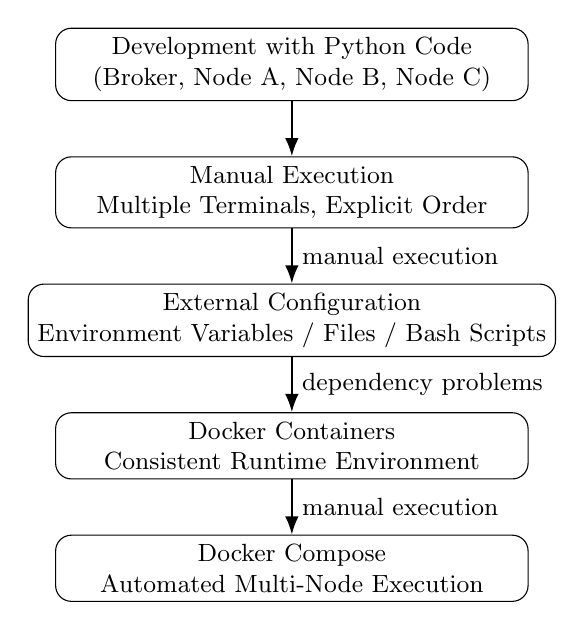
\begin{tikzpicture}[
	  font=\small,
	  node distance=7mm,
	  box/.style={
	    draw,
	    rounded corners=2mm,
	    align=center,
	    minimum width=60mm,
	    minimum height=7mm
	  },
	  arrow/.style={-Latex, thick}
	]
	
	\node[box] (code) {Development with Python Code\\(Broker, Node A, Node B, Node C)};
	\node[box, below=of code] (manual) {Manual Execution\\Multiple Terminals, Explicit Order};
	\node[box, below=of manual] (config) {External Configuration\\Environment Variables / Files / Bash Scripts};
	\node[box, below=of config] (docker) {Docker Containers\\Consistent Runtime Environment};
	\node[box, below=of docker] (compose) {Docker Compose\\Automated Multi-Node Execution};
	
	\draw[arrow] (code) -- (manual);
	\draw[arrow] (manual) -- node[right]{manual execution} (config);
	\draw[arrow] (config) -- node[right]{dependency problems} (docker);
	\draw[arrow] (docker) -- node[right]{manual execution} (compose);
	
	\end{tikzpicture}
	}
	
	\vspace{6pt}
	{\footnotesize Development and execution flow from code-level execution to container orchestration}
\end{frame}

\section{Student Activities}

	\begin{frame}{\hfill}
		\centering
		\Huge{\textbf{Student Activities}}
	\end{frame}
	
\begin{frame}{Activities for IT and Non-IT Students}
	\vspace{10pt}
	\begin{itemize}
		\item Activities are organised as \textbf{collaborative group reflections}.
		\item Each group includes at least one participant with an IT background.
		\item The goal is to combine \textbf{technical and non-technical perspectives} when observing a running system.
		\item No programming or implementation knowledge is required.
		\item Emphasis is placed on \textbf{observation, discussion, and explanation} using everyday language.
	\end{itemize}
	
	\vspace{6pt}
	{\footnotesize Focus on understanding behaviour through shared reasoning}
\end{frame}

\begin{frame}{Activities for IT Students}
	\vspace{10pt}
	\begin{itemize}
		\item Please follow and execute activities and steps presented in the moudule (Chapter 2).
		\item Hands-on activities focus on \textbf{direct execution} and \textbf{runtime reasoning}.
		\item Systems are executed at multiple levels: \textbf{raw Python processes}, \textbf{Docker CLI}, and \textbf{Docker Compose}.
		\item Configuration is modified through \textbf{environment variables}, not source code.
		\item Students observe the impact of parameter changes on \textbf{quality, performance, and behaviour}.
		\item Execution scenarios include \textbf{manual startup}, \textbf{container-based execution}, and \textbf{service scaling}.
		\item Detailed commands and step-by-step instructions are provided in the module.
	\end{itemize}
	
	\vspace{6pt}
	{\footnotesize Emphasis on execution, configuration, and operational understanding}
\end{frame}

\section{Reflection}

	\begin{frame}{\hfill}
		\centering
		\Huge{\textbf{Reflection}}
	\end{frame}
	
\begin{frame}{Group Activity: Observing and Reasoning}
	\vspace{10pt}
	\begin{enumerate}
		\item Which variables or parameters change frequently, and which remain static and repeatable?
		\item Which activities or steps are repeatedly performed when running or configuring the system?
		\item Can these repeated activities be automated, and would generation reduce effort or errors?
		\item What are the most important attributes of the system (nodes, connections, parameters, execution order)?
		\item Would a higher-level representation (configuration, DSL, or visual model) make the system easier to understand?
	\end{enumerate}
	
	\vspace{6pt}
	{\footnotesize Reflection focus: abstraction, simplification, automation, and generation}
\end{frame}

\section{Summary}
	\begin{frame}{\hfill}
		\centering
		\Huge{\textbf{Summary}}
	\end{frame}

\begin{frame}{Summary}
	\vspace{10pt}
	\begin{itemize}
		\item The course begins from \textbf{running software systems}, not from design artefacts.
		\item Observable runtime behaviour provides the foundation for system understanding.
		\item Configuration and environment significantly influence how systems behave.
		\item Manual execution exposes repetition, fragility, and operational complexity.
		\item These limitations motivate abstraction, modeling, and automation.
		\item Subsequent sessions build toward \textbf{executable models} and \textbf{automated DevSecOps}.
	\end{itemize}
	
	\vspace{6pt}
	{\footnotesize From execution and observation to abstraction and systematic design}
\end{frame}


\end{document}
